\chapter{Realisierung} \label{ch:results}

Dieses Kapitel befasst sich mit den Schritten der Realisierung dieses Projekts.

Zu Beginn wurde die \ac{db} \texttt{mii\_icu} entwickelt und die Parameter der \ac{fhir}-Profile des Erweiterungsmodul \glqq Intensivmedizin\grqq{} zusammen mit den relevanten Konfigurationsvariablen von \ac{copra} aus der \ac{copra}-Instanz des Staging Bereichs des \ac{dw} des \ac{diz} in dieser \ac{db} importiert. In dieser \ac{db} wurden die Zwischenschritten des Data Mappings realisiert, und ein Datensatz mit zugeordneten Konfigurationsvariablen mit \ac{fhir}-Profilen erzeugt. Dieser Datensatz wurde danach in den \ac{copra}-Instanz des Staging Bereichs des \ac{dw} importiert. Mit diesem Datensatz als Basis wurden \ac{sql}-Views für die Zusammenführung der Daten beider Systeme.

Ein Diagramm mit den Komponenten und dem Fluss der Daten in diesem Projekt ist in der \ref{fig:components} dargestellt.

\clearpage

\begin{figure}[ht]
	\centering
	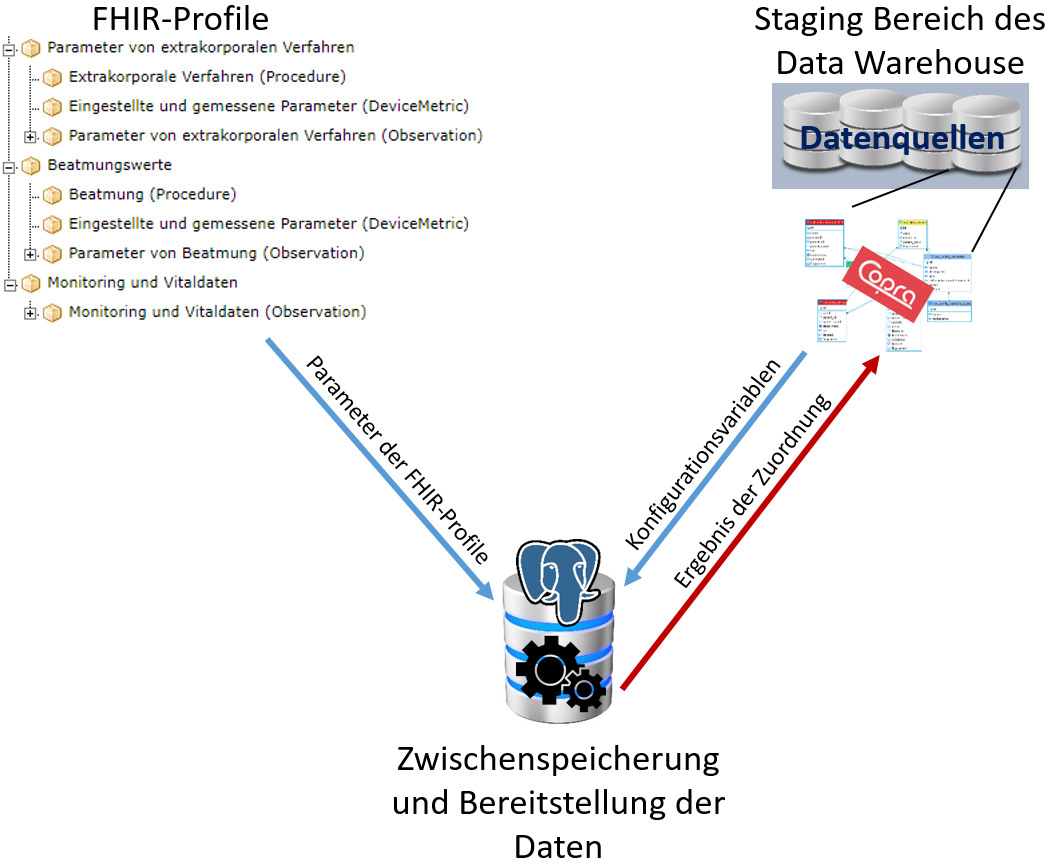
\includegraphics[height=9.5cm]{figures/master_diagram}
	\caption[Komponenten und Fluss der Daten] {Komponenten und Fluss der Daten in diesem Projekt.}
	\label{fig:components}
\end{figure}

\begin{comment}
Die Entwicklung der \ac{db} für die Speicherung und Bearbeitung der Daten wird zunächst präsentiert. Anschließend erfolgt eine Charakterisierung und Analyse der \ac{fhir}-Profile. 
Weiterhin wird die Analyse der Tabellen für das Data Mapping durchgeführt.

Danach folgt die Erläuterung der Auswahl der benutzten Konfigurationsvariablen von \ac{copra} für das Data Mapping, insbesondere für das Pattern Matching. Des Weiteren folgt die Prozedur des Pattern Matchings für die Zuordnung der \ac{fhir}-Profile mit den Konfigurationsvariablen von \ac{copra}. Zusätzlich wird die Validierung des Resultats der Zuordnung der Konfigurationsvariablen mit den \ac{fhir}-Profilen kommentiert. Nach der Validierung wird die Untersuchung der Maßeinheiten beider Systeme dargestellt. Zunächst wird die Planung und Vorbereitung für die Überführung der Daten aus \ac{copra} in die \ac{fhir}-Ressourcen mit Hilfe von programmierten \ac{sql}-Views in der \ac{copra}-Instanz des Staging Bereichs des \ac{dw} erläutert.
\end{comment}
